\begin{center}
    \Huge{\textbf{\underline{Exercise 1}}}
\end{center}

\vspace{0.6cm}

We consider the ring \( \mathbb{Z}_{34} = \{0,1,2,\dots,33\} \) of integers modulo 34.

\begin{enumerate}
    \item List all numbers in \( \mathbb{Z}_{34} \) that are coprime to 34.
    \item Find the multiplicative inverse of 3, 13, and 29 in \( \mathbb{Z}_{34} \).

Given the encryption function \(E(a, x)\) = \(x \cdot a\) mod 34

\begin{center}
    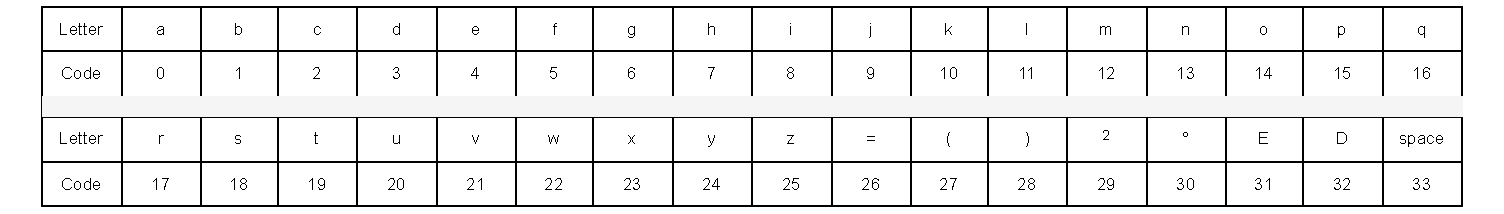
\includegraphics[width=0.9\textwidth]{Exercices/EX1/ex1.tab.drawio.pdf}
\end{center}



    \item Determine the number of possible keys.
    \item Derive the decryption function corresponding to \( E(a, x) \).
    \item Encrypt the following message using \( a = 13 \):  
        \begin{itemize}
            \item \( E = mc^2 \)
        \end{itemize}
\end{enumerate}


\vspace{1cm}
\textbf{\underline{\Large{Solution}}}\\[0.15cm]
\textbf{\underline{1. Finding All Comprime Integers Of 34}}\\[0.15cm]
\textbf{\underline{Number Of Comprime}}
\vspace{0.35cm}

\begin{center}
    34 = \(2^1 \times 17^1\)\\[0.2cm]
\(\phi(34) = 34 \times \left(1 - \frac{1}{2}\right) \times \left(1 - \frac{1}{17}\right) = \boxed{16}\)
\end{center}

\vspace{0.25cm}

There are 16 numbers coprime to 34. These numbers are not divisible by 2 or 17

\vspace{0.25cm}
\begin{center}
Coprime Numbers = \{ 1 , 3 , 5 , 7 , 9 , 11 , 13 , 15 , 19 , 21 , 23 , 25 , 27 , 29 , 31 ,33\} 
\end{center}
\vspace{1cm}
\textbf{\underline{2. Finding Multiplicative}}\\[0.15cm]
\begin{center}
    \(a^{-1}\cdot a = 34\cdot k +1\)\\[0.4cm]
    \(\boxed{a^{-1} = \dfrac{34\cdot k +1}{a}}\)
\end{center}

\newpage
\textbf{\underline{a = 3}}\\[0.15cm]
for \(k = 2\) we have :
\begin{center}
    \({a^{-1} = \dfrac{34\cdot 2 +1}{3} = \boxed{23}}\)
\end{center}

\vspace{0.5cm}

\textbf{\underline{a = 13}}\\[0.15cm]
for \(k = 8\) we have :
\begin{center}
    \({a^{-1} = \dfrac{34\cdot 8 +1}{13} = \boxed{21}}\)
\end{center}

\vspace{0.5cm}
\textbf{\underline{Euclid Methods}}\\[0.15cm]
\textbf{\underline{a = 29}}\\[0.15cm]

\begin{center}
    \(34 = 29 \times 1 + 5\)\\[0.1cm]
    \(29 = 5 \times 5 + 4\)\\[0.1cm]
    \(5 = 4 \times 1 + 1\)
\end{center}

Back-substituting to express \(1\) as a linear combination of \(34\) and \(29\):  
\[
1 = 5 - 4 \times 1
\]
\(4 = 29 - 5 \times 5\), we substitute:  
\[
1 = 5 - (29 - 5 \times 5)
\]
\(5 = 34 - 29\), we substitute: 
\begin{align*}
&1 = (34-29) - (29 - (34-29) \times 5)\\[0.1cm]
&1 = 34 - 29 - 29 + 5(34 -29)\\[0.1cm]
&1 = 34(6) + 29(\boxed{-7})
\end{align*}

Thus, the modular inverse of \(29\) modulo \(34\) is (-7 mod 34) = \(\boxed{27}\).

\vspace{1cm}
\textbf{\underline{3. Number Of Possible Keys}}\\[0.15cm]
Number of possible keys is the same as number of coprime numbers with 34 which we previously found was \(\boxed{16}\) 

\vspace{1cm}
\textbf{\underline{4. Decryption Function}}\\[0.15cm]
 \begin{center}
     \(\boxed{D(a^{-1},y) = y\cdot a^{-1} \text{ mod } 34}\)
 \end{center}

\newpage
\textbf{\underline{5. Encryption}}\\[0.15cm]

\begin{center}
    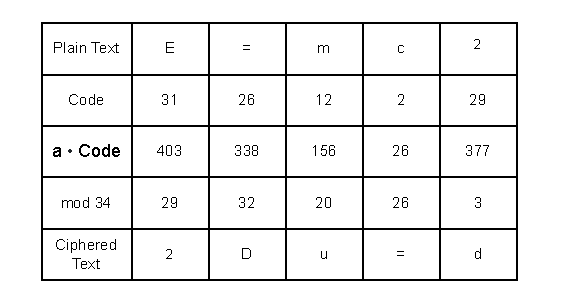
\includegraphics[height=0.3\textheight]{Exercices/EX1/encry.tab.drawio.pdf}
\end{center}


